\documentclass[]{article}

\usepackage[italian]{babel}
\usepackage[margin=20mm, footskip = 20pt]{geometry}
\usepackage{array}
\usepackage{tabularx}
\usepackage{graphicx}
\usepackage{subfiles}
\usepackage{hyperref}
\usepackage{nameref}
\usepackage{titlesec}
\usepackage{longtable}
\usepackage[table]{xcolor}
\usepackage{titling}
\usepackage{lastpage}
\usepackage{ifthen}
\usepackage{calc}
\usepackage{soulutf8}
\usepackage{contour}
\usepackage{float}
\usepackage{fancyhdr}
\usepackage{multirow}
\usepackage{pgfgantt}
\usepackage{lscape}

\newcommand{\hr}{\par\vspace{-.1\ht\strutbox}\noindent\hrulefill\par}

\graphicspath{ {./}
	{./commons/res}
}

%--------------------------------------------------
% Comandi per inserire contenuto del documento
%--------------------------------------------------
\makeatletter

\newcommand\appendToGraphicsPath[1]{%
	\g@addto@macro\Ginput@path{{#1}}%
}

\newcommand{\setTitle}[1]{%
	\newcommand{\@phTitle}{#1}%
}
\newcommand{\phTitle}{\@phTitle}

\newcommand{\setDate}[1]{%
	\newcommand{\@phDate}{#1}%
}
\newcommand{\phDate}{\@phDate}

\newcommand{\setUso}[1]{%
	\newcommand{\@uso}{#1}%
}
\newcommand{\uso}{\@uso}

\newcommand{\setVersione}[1]{%
	\newcommand{\@versione}{#1}%
}
\newcommand{\versione}{\@versione}

\newcommand{\disabilitaVersione}{%
	\renewcommand{\setVersione}[1]{}%
	\renewcommand{\versione}{DISABILITATA}
}

\newcommand{\setResponsabile}[1]{%
	\newcommand{\@responsabile}{#1}%
}
\newcommand{\responsabile}{\@responsabile}

\newcommand{\setRedattori}[1]{%
	\newcommand{\@redattori}{#1}%
}
\newcommand{\redattori}{\@redattori}

\newcommand{\setVerificatori}[1]{%
	\newcommand{\@verificatori}{#1}%
}
\newcommand{\verificatori}{\@verificatori}

\newcommand{\setModifiche}[1]{%
	\newcommand{\@modifiche}{#1}%
}
\newcommand{\modifiche}{\@modifiche}

\makeatother 

%--------------------------------------------------
% Comandi per i documenti esterni e il glossario
%--------------------------------------------------

\newcommand{\dext}[1]{\textsc{#1\textsubscript{\textit{D}}}}

\newcommand{\glock}[1]{\textsc{#1\textsubscript{\textit{G}}}}

%--------------------------------------------------
% Comandi per impostare sottotitoli di quarto e quinto livello
%--------------------------------------------------

\setcounter{secnumdepth}{4}
\setcounter{tocdepth}{4}

\titleformat{\paragraph}
{\normalfont\normalsize\bfseries}{\theparagraph}{1em}{}
\titlespacing*{\paragraph}{0pt}{2.25ex plus 1ex minus .2ex}{1.5ex plus .2ex}

\titleformat{\subparagraph}
{\normalfont\normalsize\bfseries}{\thesubparagraph}{1em}{}
\titlespacing*{\subparagraph}{0pt}{1.75ex plus 1ex minus .2ex}{.75ex plus .1ex}

\appendToGraphicsPath{../../commons/res/}

%------------------------------
%
% COMANDI DI CONFIGURAZIONE
%
%------------------------------

\setTitle{Glossario}

\setVersione{2.0.0}

\setDate{14-03-2021}

\setResponsabile{Alessandro Dindinelli}

\setRedattori{
	Alessandro Chimetto\\&
	Alessandro Dindinelli\\&
	Paolo Scanferlato}

\setVerificatori{
	Matteo Alba\\&
	Alessandro Chimetto\\&
	Valton Tahiraj}

\setUso{Esterno}

\setModifiche{
    2.0.0 & Alessandro Dindinelli & Responsabile & 14-03-2021 & Approvazione documento v2.0.0 \\
    1.3.0 & Alessandro Chimetto & Verificatore & 13-03-2021 & Verifica nuovi termini\\
	1.2.1 & Paolo Scanferlato & Amministratore & 13-03-2021 & Aggiunti tutti i termini segnalati\\
	1.2.0 & Alessandro Chimetto & Verificatore & 13-03-2021 & Verifica nuovi termini\\
	1.1.1 & Alessandro Dindinelli & Amministratore & 13-03-2021 & Aggiunti nuovi termini\\
	1.1.0 & Valton Tahiraj      & Verificatore   & 11-03-2021 & Verifica aggiunti nuovi termini \\
    1.0.1 & Alessandro Chimetto & Amministratore & 11-03-2021 & Aggiunti nuovi termini\\
	1.0.0 & Alessandro Chimetto & Responsabile & 10-01-2021 & Revisione e approvazione\\
	0.2.1 & Paolo Scanferlato & Amministratore & 09-01-2021 & Aggiunti termini norme di progetto e verbali\\
	0.2.0 & Valton Tahiraj    & Verificatore   & 06-01-2021 & Verifica termini studio di fattibilità \\
	0.1.1 & Paolo Scanferlato & Amministratore & 06-01-2021 & Aggiunti termini studio di fattibilità\\
	0.1.0 & Valton Tahiraj    & Verificatore   & 04-01-2021 & Verifica prima stesura\\
	0.0.1 & Paolo Scanferlato & Amministratore & 04-01-2021 & Prima stesura}
\begin{document}

	% Direttive per la creazione del titolo tramite comando maketitle
\title{\huge \textsc{\phTitle{}} \\
	\vspace{11pt} \large \textsc{\phDate{}}}

\author{} % Non toccare
\date{} % Non toccare

%--------------------
% Frontespizio
%--------------------

% Logo del gruppo
\begin{figure}[t!]
	\centering
	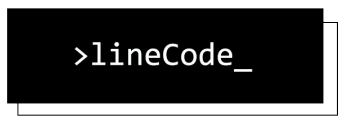
\includegraphics[width=20em]{lclong}
\end{figure}

% Titolo / Nome
\maketitle
\thispagestyle{empty}

% Dati specifici sul doc in forma tabulare
\begin{table}[ht]
	\begin{center}
		\label{tab:Dati sul documento}
		\begin{tabular}{r|l}
			\multicolumn{2}{c}{ \textsc{Dati sul documento} } \\
			\hline
			\textbf{Versione} & \versione{} \\
			\textbf{Uso} & \uso{}  \\
			\textbf{Redattori} & \redattori{} \\
			\textbf{Verificatori} & \verificatori{} \\
			\textbf{Responsabile} & \responsabile{} \\
			\textbf{Destinatari} & lineCode \\
								& prof.\ Vardanega Tullio \\		
								& prof.\ Cardin Riccardo \\
			\ifthenelse{\equal{\uso}{Esterno}}{
								& Sanmarco Informatica
			}{} \\
		\end{tabular}
	\end{center}
\end{table}

\newpage

\renewcommand{\arraystretch}{2} % allarga le righe con dello spazio sotto e sopra
\begin{longtable}[H]{>{\centering\bfseries}m{2cm} >{\centering}m{3.5cm} >{\centering}m{2.5cm} >{\centering}m{3cm} >{\centering\arraybackslash}m{5cm}}
	\rowcolor{lightgray}
	{\textbf{Versione}} & {\textbf{Nominativo}} & {\textbf{Ruolo}} & {\textbf{Data}} & {\textbf{Descrizione}}  \\
	\endfirsthead%
	\rowcolor{lightgray}
	{\textbf{Versione}} & {\textbf{Nominativo}}  & {\textbf{Ruolo}} & {\textbf{Data}} & {\textbf{Descrizione}}  \\
	\endhead%
	\modifiche{}%
\end{longtable}
	\newpage

	\tableofcontents

	\newpage
	\phantomsection
	\addcontentsline{toc}{section}{A}

	\section*{A}

	\paragraph*{Act}
	Tool per utilizzare le Github Actions in locale.

	\paragraph*{Amazon CloudWatch}
	Servizio di monitoraggio e osservabilità delle risorse e applicazioni AWS su AWS e sui server locali. Fornisce dati e analisi concrete per monitorare le applicazioni, rispondere ai cambiamenti di prestazioni a livello di sistema, ottimizzare l'utilizzo delle risorse e ottenere una visualizzazione unificata dello stato di integrità operativa.

	\paragraph*{Amazon Cognito}
	Servizio di Amazon Web Service che permette di aggiungere strumenti di registrazione, accesso e controllo degli accessi alle applicazioni Web e per dispositivi mobili.

	\paragraph*{Amazon Gamelift}
	È una soluzione di hosting di server di giochi che distribuisce, gestisce e dimensiona i server cloud per giochi multigiocatore.

	\paragraph*{Amazon Web Service}
	Vedere AWS.

	\paragraph*{Angular o Angular2+}
	Framework open source per lo sviluppo di applicazioni web con licenza MIT, evoluzione di AngularJS.

	\paragraph*{AngularJS}
	Prima versione di un Framework open source per lo sviluppo di applicazioni web. Nel 2016 si è evoluto in Angular2+.

	\paragraph*{API}
	Con Application Programming Interface si intende un insieme di procedure e funzioni offerte ai programmatori per facilitare lo sviluppo. Le API espongono blocchi di codice delle librerie di cui fanno parte, per permetterne il riuso.

	\paragraph*{API Rest}
	Sono un set di API che rispettano il modello architetturale REST.

	\paragraph*{Android}
	Sistema operativo per dispositivi mobili sviluppato da Google Inc., basato su kernel Linux in cui la quasi totalità delle utilità sono costituite da software Java.

	\paragraph*{Atmosphere}
	È un framework per lo sviluppo di applicazioni web in Java asincrone e real time che implementa vari meccanismi di push technology.

	\paragraph*{Automated Kanban}
	Bacheca in stile Kanban con trigger integrati per spostare automaticamente gli issue e sistemarli nelle colonne To do, In progress e Done.

	\paragraph*{AWS}
	Amazon Web Services, è una collezione di servizi di cloud computing che compongono la piattaforma on-demand di servizi, offerta da Amazon.	Comprende servizi di calcolo, di rete e di storage di basi di dati oltre a molti altri servizi.

	\paragraph*{AWS Appsync}
	Servizio completamente gestito che facilita lo sviluppo di API GraphQL gestendo le attività impegnative derivanti dalla connessione sicura a origini dati come AWS Lambda.

	\paragraph*{AWS Lambda}
	Servizio di elaborazione che consente di eseguire il codice senza gestire i server o effettuarne il provisioning.

	\newpage
	\phantomsection
	\addcontentsline{toc}{section}{B}

	\section*{B}

	\paragraph*{Back-end}
	Indica generalmente l'interfaccia amministrativa di un applicativo o di un sito web.

	\paragraph*{Big Data}
	Una raccolta di dati molto estesa in termini di	volume, velocità e varietà da richiedere tecnologie e metodi analitici specifici per l'estrazione di valore o conoscenza.

	\paragraph*{Blockchain}
	Struttura dati condivisa e immutabile. È definita come un registro digitale le cui voci sono raggruppate in blocchi, concatenati in ordine cronologico, e la cui integrità è garantita dall'uso della crittografia.

	\paragraph*{Bluetooth}
	Standard tecnico-industriale di trasmissione dati per reti personali senza fili.

	\paragraph*{Branch}
	Indica un ramo di sviluppo in un Version Control System.

	\paragraph*{Browser}
	Applicazione per l'acquisizione, la presentazione e la navigazione di risorse sul web.

	\paragraph*{Build Automation}
	Scrivere o automatizzare un'ampia varietà di compiti che gli sviluppatori software fanno nelle loro attività quotidiane di sviluppo: compilazione, pacchettizzazione, esecuzione dei test, deployment e creazione di documentazione e/o note di rilascio.

	\newpage
	\phantomsection
	\addcontentsline{toc}{section}{C}

	\section*{C}

	\paragraph*{C}
	Linguaggio di programmazione imperativo di natura procedurale; i programmi scritti in questo linguaggio sono composti da espressioni matematiche e da istruzioni imperative raggruppate in procedure parametrizzate in grado di manipolare vari tipi di dati.

	\paragraph*{C++}
	Linguaggio di programmazione general-purpose, sviluppato come evoluzione del linguaggio C inserendo la programmazione orientata agli oggetti, col tempo ha avuto notevoli evoluzioni, come l'introduzione dell'astrazione rispetto al tipo.

	\paragraph*{Canva}
	Strumento di progettazione grafica.

	\paragraph*{Capitolato}
	Documento tecnico redatto dal cliente in cui vengono specificati i vincoli contrattuali	(prezzo e scadenze) per lo sviluppo di un determinato prodotto software. Viene presentato in un bando d'appalto per trovare qualcuno che possa svolgere il lavoro richiesto.

	\paragraph*{Checkstyle}
	Strumento di sviluppo per automatizzare il processo di controllo del codice Java. Aiuta a scrivere codice conforme a delle code conventions ben definite.

	\paragraph*{CI}
	Continuous Integration, è una pratica che si applica in contesti in cui lo sviluppo del software avviene attraverso un sistema di controllo versione.

	\paragraph*{Cloud}
	Indica un paradigma di erogazione di servizi offerti on-demand da un fornitore ad un cliente finale attraverso la rete Internet.

	\paragraph*{Code Coverage}
	Misura utilizzata per descrivere il grado in cui viene eseguito il codice sorgente di un programma quando viene eseguita una particolare suite di test.

	\paragraph*{Code-review}
	Attività di garanzia della qualità del software in cui una o più persone controllano un programma principalmente visualizzando e leggendo parti del suo codice sorgente e lo fanno dopo l'implementazione o come interruzione dell'implementazione.

	\paragraph*{Commit}
	In questo contesto si riferisce ad una o più modifiche effettuate in una repository, a cui viene associato un nome e un codice identificativo per il tracciamento.

	\paragraph*{Container(Docker)}
	Applicazione isolata (con tutte le sue dipendenze) eseguita in namespace separati.

	\paragraph*{Continuous Integration}
	Pratica che si applica in contesti in cui lo sviluppo del software avviene attraverso un sistema di controllo versione. Consiste nell'allineamento frequente dagli ambienti di lavoro degli sviluppatori verso l'ambiente condiviso.

	\paragraph*{CSS}
	Cascaded Style Sheet, è un linguaggio che permette di definire tutte le proprietà di stile e formattazione di una pagina web in maniera modulare, tenendo questa parte della progettazione di un sito separata da quella relativa al contenuto.

	\paragraph*{CSV}
	Comma-Separated Values, è un formato di file basato su file di testo utilizzato per l'importazione ed esportazione (ad esempio da fogli elettronici o database) di una tabella di dati.

	\newpage
	\phantomsection
	\addcontentsline{toc}{section}{D}

	\section*{D}

	\paragraph*{D3.js}
	Libreria JavaScript per creare visualizzazioni dinamiche ed interattive partendo da dati organizzati, visibili attraverso un comune browser.

	\paragraph*{Deploy}
	In informatica è la consegna o rilascio al cliente, con relativa installazione e messa in funzione o esercizio, di una applicazione o di un sistema software tipicamente all’interno di un sistema informatico aziendale.

	\paragraph*{Design Pattern}
	Soluzione progettuale generale a un problema ricorrente. È la descrizione di un modello da applicare per risolvere un problema, il quale può presentarsi in diverse situazioni durante la progettazione e lo sviluppo del software. Ogni design pattern ha il suo campo applicativo in base alle precondizioni del problema, coi suoi pregi e difetti.

	\paragraph*{DevOps}
	Metodo di sviluppo del software che punta alla comunicazione, collaborazione e integrazione tra sviluppatori e addetti alle operations della Information Technology.

	\paragraph*{Diagrams}
	Software on-line per la creazione di diagrammi.

	\paragraph*{Discord}
	Applicazione VoIP originariamente progettata per le comunità di videogiocatori.

	\paragraph*{Docker}
	Progetto open-source che automatizza la distribuzione di applicazioni all'interno di contenitori software, fornendo un'astrazione aggiuntiva grazie alla virtualizzazione a livello di sistema operativo di Linux.

	\paragraph*{Dockerfile}
	In Docker, è un documento di testo che contiene tutti i comandi che un utente può chiamare sulla riga di comando per assemblare un'immagine.

	\paragraph*{Docker Compose}
	Strumento per la definizione e l’esecuzione di applicazioni Docker multi-contenitore. Tramite un file Compose è possibile utilizzare un singolo comando per creare e avviare tutti i servizi di una configurazione.

    \paragraph*{Drive}
    È un servizio web di Google, in ambiente \glock{cloud}, di memorizzazione e sincronizzazione di file online.

	\paragraph*{DVCS}
	Distributed Version Control Systems, è una tipologia di controllo di versione che permette di tenere traccia delle modifiche e delle versioni apportate al codice sorgente del software.

	\newpage
	\phantomsection
	\addcontentsline{toc}{section}{E}

	\section*{E}

	\paragraph*{E-commerce}
	Pratica commerciale che mette in contatto commercianti e acquirenti tramite Internet. Le transazioni di beni e/o servizi vengono effettuate da un negozio online, da un'applicazione mobile e da altri canali di vendita come social network, marketplace, piattaforme di affiliazione, siti di compravendita, ecc.

	\paragraph*{Ethereum}
	Ethereum è una piattaforma decentralizzata per la creazione e pubblicazione peer-to-peer di contratti intelligenti (smart contracts).

	\paragraph*{Exploratory Data Analysis}
	Spesso abbreviato in EDA, è una tecnica usata nel campo della Data Science per approfondire la conoscenza del dataset su cui si intende lavorare, operazione cruciale per svolgere su di esso qualsiasi tipo di attività.

	\newpage
	\phantomsection
	\addcontentsline{toc}{section}{F}

	\section*{F}

	\paragraph*{Feature Branch}
	I Feature Branch nei sistemi di VCS consentono di lavorare su una funzionalità indipendentemente dallo sviluppo principale e di eseguire il commit di tutte le modifiche per la funzionalità nel branch, unendo le modifiche nel branch principale quando la funzionalità è completa.

	\paragraph*{Force Field}
	Tipologia di rappresentazione grafica di dati.

	\paragraph*{Framework}
	Architettura logica di supporto (spesso un'implementazione logica di un particolare design pattern) su cui un software può essere progettato e realizzato, spesso facilitandone lo sviluppo da parte del programmatore.

	\paragraph*{Front-end}
	Indica generalmente l'interfaccia utente di un applicativo o sito web.

	\newpage
	\phantomsection
	\addcontentsline{toc}{section}{G}

	\section*{G}

	\paragraph*{Gantt}
	Il diagramma di Gantt è uno strumento di supporto alla gestione dei progetti, così chiamato in ricordo dell'ingegnere statunitense Henry Lawrence Gantt (1861-1919), che si occupava di scienze sociali e che lo ideò nel 1917.

	\paragraph*{GanttProject}
	Software Open Source per la realizzazione dei diagrammi di Gantt.

	\paragraph*{GGobi}
	Strumento software statistico gratuito per la visualizzazione interattiva dei dati.

	\paragraph*{Git}
	Software di controllo versione distribuito utilizzabile da interfaccia a riga di comando.

	\paragraph*{Gitflow}
	Insieme di strategie sul come utilizzare Git e i suoi branch.

	\paragraph*{GitHub}
	Servizio web di hosting per lo sviluppo di progetti software che usa il sistema di controllo di versione Git.

	\paragraph*{GitHub Actions}
	Strumento fornito da GitHub che permette l’automazione di compiti di varia natura.

	\paragraph*{GitKraken}
	Client Git semplice e intuitivo che rende il più semplice possibile aprire, creare e clonare repository, creare filiali e condividere il codice.

	\paragraph*{Gmail}
	Servizio gratuito di posta elettronica fornito da Google.

    \paragraph*{Google Chat}
    Google Chat è un software di comunicazione, sviluppato da Google, creato per i team che fornisce messaggi diretti e chat room di gruppo.

    \paragraph*{Google Drive}
    Vedere Drive.

    \paragraph*{Google Meet}
    Vedere Meet.

	\paragraph*{GraphQL}
	Linguaggio di interrogazione lato server per interfacce di programmazione delle applicazioni, in grado di fornire ai client unicamente i dati di cui hanno bisogno.

	\paragraph*{Grizzly}
	Framework progettato da Oracle per aiutare gli sviluppatori a sfruttare l'API Java NIO.

	\paragraph*{gRPC}
	Sistema di chiamata di procedura remota open source sviluppato inizialmente da Google.

	\paragraph*{Gulpease}
	L'Indice Gulpease è un indice di leggibilità di un testo tarato sulla lingua italiana. Rispetto ad altri ha il vantaggio di utilizzare la lunghezza delle parole in lettere anziché in sillabe, semplificandone il calcolo automatico.

	\newpage
	\phantomsection
	\addcontentsline{toc}{section}{H}

	\section*{H}

	\paragraph*{Heat Map}
	Rappresentazione grafica dei dati dove i singoli valori contenuti in una matrice sono rappresentati da colori.

	\paragraph*{HTML}
	Linguaggio di markup per la strutturazione delle pagine web.

	\paragraph*{HTTP}
	Hypertext Transfer Protocol, è un protocollo a livello applicativo usato come principale sistema per la trasmissione d'informazioni sul web ovvero in un'architettura tipica client-server.

	\newpage
	\phantomsection
	\addcontentsline{toc}{section}{I}

	\section*{I}

	\paragraph*{IA}
	L'Intelligenza Artificiale è una disciplina appartenente all'informatica che studia i fondamenti teorici, le metodologie e le tecniche che consentono la progettazione di sistemi hardware e sistemi di programmi software capaci di fornire all'elaboratore elettronico prestazioni che, a un osservatore comune, sembrerebbero essere di pertinenza esclusiva dell'intelligenza umana.

	\paragraph*{IDE}
	Integrated Development Environment, è un ambiente di sviluppo ovvero un software che, in fase di programmazione, supporta i programmatori nello sviluppo e debugging del codice sorgente di un programma.

    \paragraph*{In-memory Database}
    Con il termine in-memory database, o main memory database system, o memory-resident database, si intende un DBMS che gestisce i dati nella memoria centrale. Esso è in contrasto con i DBMS che mantengono i dati su memorie di massa.

	\paragraph*{Inspection}
	Metodo di verifica che prevede la rilevazione di difetti eseguendo una lettura mirata (tramite check-list) dell'oggetto di verifica.

	\paragraph*{IntelliJ IDEA}
	Ambiente di sviluppo integrato per il linguaggio di programmazione Java.

	\paragraph*{iOS}
	Sistema operativo mobile sviluppato da Apple per iPhone, iPod touch e iPad.

	\paragraph*{Issue}
	È una qualsiasi richiesta o azione da svolgere in un Issue Tracking System.

	\paragraph*{Issue Tracking System}
	Software utilizzato per gestire in modo organizzato i problemi di prodotti o servizi segnalati dall’utente e giungere alla loro risoluzione.

	\newpage
	\phantomsection
	\addcontentsline{toc}{section}{J}

	\section*{J}

    \paragraph*{Jackson}
    Libreria ad alte prestazioni per Java che processa istanze trasformandole in JSON e viceversa.

	\paragraph*{JaCoCo}
	Libreria di Code Coverage gratuita per Java. Fornisce una libreria leggera, flessibile e ben documentata per l'integrazione con vari strumenti di compilazione e sviluppo.

	\paragraph*{Java}
	Linguaggio di programmazione ad alto livello, orientato agli oggetti e a tipizzazione statica, che si appoggia sull'omonima piattaforma software di esecuzione, specificamente progettato per essere il più possibile indipendente dalla piattaforma hardware di esecuzione tramite l'utilizzo di macchina virtuale.

	\paragraph*{JavaScript}
	Linguaggio di scripting orientato agli oggetti e agli eventi, utilizzato nella programmazione Web sia lato client che server.

	\paragraph*{Jersey}
	Framework Java che consente di sviluppare servizi RESTful in Java. Fornisce il supporto alla JAX-RS API e offre un’implementazione della specifica JAX-RS. Supportando una varietà di formati, consente allo sviluppatore di astrarre dai dettagli di basso livello necessari alla comunicazione client-server.

    \paragraph*{JSON}
    Acronimo di JavaScript Object Notation, è un formato adatto all'interscambio di dati fra applicazioni client/server.

	\paragraph*{JUnit}
	Framework di unit testing per il linguaggio di programmazione Java.

	\newpage
	\phantomsection
	\addcontentsline{toc}{section}{K}

	\section*{K}

	\paragraph*{Karma}
	Test runner sviluppato dal team di AngularJS

	\paragraph*{Kotlin}
	Linguaggio di programmazione general purpose, multi-paradigma, open source sviluppato dall'azienda di software JetBrains.

	\paragraph*{Kubernetes}
	Sistema open source di orchestrazione e gestione di container.

	\newpage
	\phantomsection
	\addcontentsline{toc}{section}{L}

	\section*{L}

	\paragraph*{LaTeX}
	Linguaggio di markup per la preparazione di testi, basato sul programma di composizione tipografica TEX.

	\paragraph*{Leaflet}
	Libreria JavaScript per sviluppare mappe geografiche interattive.

	\paragraph*{Learning Vector Quantization}
	Algoritmo di classificazione supervisionato basato su prototipo.

	\paragraph*{Libreoffice Calc}
	Un foglio elettronico, simile a Microsoft Excel o Lotus 1-2-3. Ha un certo numero di caratteristiche uniche, tra cui un sistema che definisce automaticamente la serie di grafici, sulla base delle informazioni disponibili per l'utente.

	\paragraph*{Linux}
	Famiglia di sistemi operativi open source di tipo Unix-like, pubblicati in varie distribuzioni, aventi la caratteristica comune di utilizzare come nucleo il kernel Linux.

	\newpage
	\phantomsection
	\addcontentsline{toc}{section}{M}

	\section*{M}

	\paragraph*{macOS}
	Sistema operativo desktop distribuito da Apple Inc. per	computer Macintosh che fornisce l'interfaccia utente caratteristica dei sistemi	MacOS ad un sistema operativo di derivazione Unix.

	\paragraph*{Major release}
	Con major release si intende una versione di un prodotto che si discosta sostanzialmente dalla versione precedente.

	\paragraph*{MAPI}
	Architettura di messaggistica basata sulle API per Microsoft Windows.

	\paragraph*{Maven}
	Strumento completo per la gestione di progetti software Java, in termini di compilazione del codice, distribuzione, documentazione e collaborazione del team di sviluppo.

	\paragraph*{Meet}
	Strumento delle Google Suite per tenere riunioni video con persone interne o esterne all'organizzazione.

	\paragraph*{Merge}
	In un VCS è l'attività che unisce più versioni dello stesso software.

	\paragraph*{Milestone}
	Termine utilizzato nella pianificazione e gestione di progetti complessi per indicare il raggiungimento di obiettivi stabiliti in fase di definizione del progetto stesso.

	\paragraph*{Minor release}
	Con minor release, si intende una specifica versione di un prodotto nella quale le differenze con la versione precedente riguardano principalmente correzioni.

	\paragraph*{Modello a V}
	Modello di sviluppo del software, estensione del modello a cascata. Il modello invece di discendere lungo una linea retta, dopo la fase di programmazione risale con una tipica forma a V.

    \paragraph*{Mock}
    Oggetto fittizio che ritorna risultati preimpostati, utilizzato nei test per isolare un'unità dal resto del sistema.

	\paragraph*{Mockito}
	Framework di per la creazione di oggetti mock per i test, open source, per Java.

	\paragraph*{MQTT}
	Protocollo ISO standard di messaggistica leggero di tipo publish-subscribe posizionato in cima a TCP/IP.

	\paragraph*{Multiplayer}
	Modalità di utilizzo in cui più persone partecipano al gioco nello stesso tempo, per mezzo di un solo apparecchio (computer, console, dispositivo mobile, ecc.) con più periferiche oppure usando diversi apparecchi in connessione.

	\newpage
	\phantomsection
	\addcontentsline{toc}{section}{N}

	\section*{N}

	\paragraph*{Node.js}
	Runtime di JavaScript Open source multipiattaforma orientato agli eventi per l'esecuzione di codice JavaScript.

	\paragraph*{Next.js}
	Framework web di sviluppo front-end React open source che abilita funzionalità come il rendering lato server e la generazione di siti web statici per applicazioni web basate su React.

	\paragraph*{NoSQL}
	Movimento che promuove sistemi software dove la persistenza dei dati è in generale caratterizzata dal fatto di non utilizzare il modello relazionale, di solito usato dalle basi di dati tradizionali.

	\paragraph*{Npm}
	Node Package Manager, è un gestore di pacchetti per il linguaggio di programmazione JavaScript. È il gestore di pacchetti predefinito per l'ambiente di runtime JavaScript Node.js. Consiste in un client da linea di comando, chiamato anch'esso npm e un database online di pacchetti pubblici e privati, chiamato npm registry.

	\newpage
	\phantomsection
	\addcontentsline{toc}{section}{O}

	\section*{O}

	\paragraph*{Openshift}
	Piattaforma container per le imprese basata su Kubernetes, che offre operazioni automatizzate in tutto lo stack per gestire deployment di cloud ibridi e multicloud.

	\paragraph*{Open Source}
	Software non protetto da copyright, che segue la filosofia della produzione collaborativa e dell'accesso pubblico al codice sorgente.

	\paragraph*{Orange Canvas}
	Toolkit di visualizzazione dati, machine learning e data mining open source.

	\newpage
	\phantomsection
	\addcontentsline{toc}{section}{P}

	\section*{P}

	\paragraph*{Patch}
	Piccola parte di software utilizzata per aggiornare o migliorare un programma e correggere un problema di vulnerabilità di sicurezza, di solito chiamato bug, all'interno di un sistema operativo o di un programma software.

	\paragraph*{PDF}
	Portable Document Format, è un formato di file basato su un linguaggio di descrizione di pagina sviluppato da Adobe negli anni 1990 per rappresentare documenti di testo e immagini in modo indipendente dall'hardware e dal software utilizzati per generarli o per visualizzarli.

	\paragraph*{PHP}
	Hypertext Preprocessor, è un linguaggio di scripting interpretato, originariamente concepito per la programmazione di pagine web dinamiche.

	\paragraph*{POI}
	Point Of Interest, è un punto specifico che qualcuno potrebbe trovare utile o interessante.

    \paragraph*{Power-up}
    Nei videogiochi, è un oggetto mostrato a video che conferisce una particolare abilità temporanea (limitata nel tempo) al giocatore o ne incrementa le statistiche quando raccolto.

	\paragraph*{Product Baseline}
	Baseline del progetto di ingegneria del software in cui il prodotto è stato realizzato e funziona, ma non è ancora pronto per il rilascio.

	\paragraph*{Proiezione Lineare Multi Asse}
	Tipologia di rappresentazione grafica di dati.

	\paragraph*{Proof of Concept}
	Realizzazione incompleta o abbozzata (prototipo) di un determinato progetto o metodo, allo scopo di fornire la dimostrazione pratica dei funzionamenti di base di un applicativo o di un intero sistema.

	\paragraph*{Protractor}
	Framework di test end-to-end per applicazioni Angular e Angular JS.

	\paragraph*{Publisher/Subscriber}
	Stile architetturale utilizzato per la comunicazione asincrona fra diversi processi, oggetti o altri agenti.

	\paragraph*{Pull-Request}
	Richiesta di salvataggio delle modifiche in un branch del Version Control System.

	\paragraph*{Python}
	Linguaggio di programmazione di più "alto livello" rispetto alla maggior parte degli altri linguaggi, orientato a oggetti, adatto, tra gli altri usi, a sviluppare applicazioni distribuite, scripting, computazione numerica e system testing.

	\newpage
	\phantomsection
	\addcontentsline{toc}{section}{Q}

	\section*{Q}

	\paragraph*{Qt Framework}
	Libreria multipiattaforma per lo sviluppo di programmi con interfaccia grafica tramite l'uso di widget.

	\paragraph*{Query}
	Indica l'interrogazione da parte di un utente su un database, strutturato tipicamente secondo il modello relazionale, per compiere determinate operazioni sui dati.

	\newpage
	\phantomsection
	\addcontentsline{toc}{section}{R}

	\section*{R}

	\paragraph*{Rancher}
	Piattaforma di orchestrazione open source che permette il rilascio e la gestione di Kubernetes.

	\paragraph*{React}
	Libreria JavaScript per la creazione di interfacce utente.

	\paragraph*{Real-Time}
	Un sistema real-time è un calcolatore in cui la correttezza del risultato delle sue computazioni dipende non solo dalla correttezza logica ma anche dalla correttezza temporale.

    \paragraph*{Redis}
    Database chiave-valore open-source residente in memoria con persistenza facoltativa.

	\paragraph*{Release}
	Ciascuna nuova versione di un software, messa in commercio o comunque diffusa, contraddistinta da un numero.

	\paragraph*{Repository}
	Ambiente di un sistema informativo, in cui vengono gestiti i metadati, attraverso tabelle relazionali.

	\paragraph*{RFID}
	Radio-Frequency IDentification, è la tecnologia di identificazione automatica basata sulla propagazione nell'aria di onde elettro-magnetiche, consentendo la rilevazione univoca, automatica (hand free), massiva e a distanza di oggetti, animali e persone sia statici che in movimento.

	\paragraph*{Root}
	Il punto iniziale del file system. Il nome deriva dal riferimento alla sua organizzazione ad albero (quindi alla sua radice) comune a molti file system.

	\newpage
	\phantomsection
	\addcontentsline{toc}{section}{S}

	\section*{S}

	\paragraph*{Scatter Plot Matrix}
	È una griglia (o matrice) di grafici a dispersione utilizzati per visualizzare le relazioni di una coppia di variabili tra combinazioni di variabili.

	\paragraph*{Self Organizing Map}
	Tipo di organizzazione di processi di informazione in rete analoghi alle reti neurali artificiali.

	\paragraph*{SEO}
	Search Engine Optimization, definisce tutte le attività di ottimizzazione di un sito web volte a migliorarne il posizionamento nei risultati organici dei motori di ricerca.

    \paragraph*{Sig4j}
    Libreria Java per l'impostazione di un sistema signal/slot simile a quello della libreria grafica Qt per C++.

	\paragraph*{Singleplayer}
	Nel mondo dei videogiochi indica la modalità di gioco in cui una sola persona prende parte al gioco per tutta la durata della partita.

	\paragraph*{Smart Contract}
	Gli Smart Contract sono protocolli informatici che facilitano, verificano, o fanno rispettare, la negoziazione o l'esecuzione di un contratto, permettendo talvolta la parziale o la totale esclusione di una clausola contrattuale. Di solito, hanno anche un'interfaccia utente e spesso simulano la logica delle clausole contrattuali.

	\paragraph*{Solidity}
	Linguaggio di programmazione orientato agli oggetti per scrivere contratti intelligenti. Viene utilizzato per implementare contratti intelligenti su varie piattaforme Blockchain, in particolare Ethereum.

    \paragraph*{SonarCloud}
    Servizio Cloud per la misurazione della qualità di un prodotto software tramite analisi statica del codice.

	\paragraph*{SQL}
	Linguaggio standardizzato per database basati sul modello relazionale, progettato per creare e modificare schemi di database; inserire, modificare e gestire dati memorizzati; interrogare i dati memorizzati; creare e gestire strumenti di controllo e accesso ai dati.

	\paragraph*{Swift}
	Linguaggio di programmazione orientato agli oggetti per sistemi macOS, iOS, watchOS, tvOS e Linux. È concepito per coesistere con il linguaggio Objective-C, tipico degli sviluppi per i sistemi operativi Apple, semplificando la scrittura del codice.
	
	\paragraph*{Subject}
	Tipo speciale di Observable per inviare dati ai components o service. A differenza degli Observable, può fare multicast su più Observer.	

	\newpage
	\phantomsection
	\addcontentsline{toc}{section}{T}

	\section*{T}

	\paragraph*{Technology Baseline}
	Definisce le tecnologie, i framework e le librerie selezionate per lo sviluppo del prodotto.

	\paragraph*{Texmaker}
	Editor LaTeX open source multipiattaforma.

	\paragraph*{TeXstudio}
	Editor LaTeX open source multipiattaforma.

	\paragraph*{Thread}
	È una suddivisione di un processo in due o più filoni o sottoprocessi che vengono eseguiti concorrentemente da un sistema di elaborazione monoprocessore o multiprocessore o multicore.

	\paragraph*{Tomcat}
	Apache Tomcat è un server web open source sviluppato dalla Apache Software Foundation.

	\paragraph*{t-SNE}
	Algoritmo di riduzione della dimensionalità ampiamente utilizzato come strumento di apprendimento automatico in molti ambiti di ricerca.

	\paragraph*{TSLint}
	Strumento che permette di fare analisi statica del codice verificandone il rispetto di un determinato stile di scrittura.

	\paragraph*{Typescript}
	Liguaggio di programmazione open-source sviluppato da Microsoft che estende il linguaggio Javascript aggiungendo alcuni costrutti sintattici.

	\newpage
	\phantomsection
	\addcontentsline{toc}{section}{U}

	\section*{U}

	\paragraph*{Underscore}
	Il trattino basso è il carattere "\_".

	\paragraph*{User-friendly}
	Indica qualcosa che è stata progettata per essere estremamente facile da usare, anche per chi non è molto pratico.

	\paragraph*{User-interface}
	Interfaccia uomo-macchina, ovvero ciò che si frappone tra una macchina e un utente, consentendone l'interazione reciproca.

	\paragraph*{UMAP}
	Piattaforma che fornisce una interfaccia grafica di semplice utilizzo per personalizzare mappe e geolocalizzare dataset appositamente creati o recuperati negli archivi Open Data.

	\paragraph*{UML}
	Unified Modeling Language, è un vero e proprio linguaggio grafico che serve per spiegare la struttura delle classi di un progetto, o più in generale del progetto stesso, in modo rapido, formale e astratto.

	\paragraph*{Unit testing}
	Attività di testing di singole unità software.

	\newpage
	\phantomsection
	\addcontentsline{toc}{section}{V}

	\section*{V}

	\paragraph*{VCS}
	Version Control System, è un sistema per la gestione delle versioni di un prodotto.

	\paragraph*{Vyper}
	Linguaggio di programmazione, basato su Python, orientato al contratto che prende di mira la Ethereum Virtual Machine (EVM).

	\newpage
	\phantomsection
	\addcontentsline{toc}{section}{W}

	\section*{W}

	\paragraph*{Walkthrough}
	Metodo di verifica che prevede la rilevazione di difetti attraverso una lettura critica ad ampio spettro del prodotto in esame.

	\paragraph*{WebSocket}
	È una tecnologia web che fornisce canali di comunicazione full-duplex attraverso una singola connessione TCP.

	\paragraph*{Windows}
	Famiglia di ambienti operativi e sistemi operativi prodotta da Microsoft Corporation dal 1985, orientato a personal computer, workstation, server e smartphone; prende il nome dall'interfaccia di programmazione di un'applicazione a finestre, detta File Explorer.

	\paragraph*{Workflow}
	Rappresenta un insieme di compiti e di diversi attori coinvolti nella realizzazione di un processo lavorativo.

	\newpage
	\phantomsection
	\addcontentsline{toc}{section}{Z}

	\section*{Z}

	\paragraph*{Zapier}
	Tool di automation erogato online come servizio dalla Zapier INC.

	\paragraph*{Zero downtime}
	Si intende un hardware o un software che non ha tempi di inattività.

	\paragraph*{Zextras Drive}
	Tecnologia della Zextras Suite che permette l'archiviazione di file nel cloud Zextras.

\end{document}